\documentclass[11pt,fleqn, twoside, final]{book}%\documentclass[12pt, openany]{book} % --- , openany,usenames,dvipsnames
\usepackage{changepage} % Para ajustar los márgenes localmente
%=============================== Preâmbulo ============================================
\usepackage{amsfonts}
\usepackage[utf8]{inputenc}
\usepackage[T1]{fontenc}
\usepackage[portuguese]{babel}
% \usepackage[latin1]{inputenc}		% Inclusão de gráficos
\usepackage[table]{xcolor}% http://ctan.org/pkg/xcolor
\usepackage{indentfirst}
\usepackage{subfigure}
\usepackage{natbib} %usepackage{harvard}
\usepackage{amssymb,fancyhdr,fancybox,epsfig,psfrag,tabularx}
\usepackage{comment}
\usepackage{amsthm}
\usepackage{graphicx}
\usepackage{footnote}
\usepackage{float}
\usepackage{hyperref}
\usepackage{amsmath}
\usepackage{pslatex}
\usepackage{algpseudocode}
\usepackage[ruled,vlined]{algorithm2e}
\usepackage{colortbl}
\definecolor{firebrick}{rgb}{.7, .13, .13}
\definecolor{lightcopper}{rgb}{.93, .76, .58}
\definecolor{blueice}{rgb}{.85, .96, .94}
\usepackage{pdfpages}


\hypersetup{
    colorlinks=true,
    citecolor=blue,
    linkcolor=blue,
    filecolor=magenta,      
    urlcolor=cyan,
}
\usepackage{booktabs}
\usepackage{multirow}
\usepackage{setspace}
\usepackage{tikz}
\usepackage{soul}
\usepackage{rotating}
\usetikzlibrary{patterns}
\usetikzlibrary{plotmarks}


\urlstyle{same}
\renewcommand\qedsymbol{$\blacksquare$}
%\usepackage[paperwidth=8.5in,paperheight=11in,hmargin={25mm,20mm},vmargin={20mm,20mm}]{geometry} %Papel Carta
%\usepackage[ruled]{algpseudocode,algorithm2e}
\usepackage[a4paper,hmargin={25mm,20mm},vmargin={20mm,20mm}]{geometry} %Papel A4
\usepackage{setspace}
\usepackage{caption}

\usepackage[Sonny]{fncychap} %Options: Sonny, Lenny, Glenn, Conny, Rejne, Bjarne, Bjornstrup
%\ChNameVar{\large\sf} \ChNumVar{\Large} \ChTitleVar{\Large\sf\raggedleft}
%\ChRuleWidth{0.24pt} \ChNameUpperCase

\setlength{\headheight}{15pt}
\usepackage[title,titletoc,toc]{appendix}

%\usepackage{proof}
%\newtheorem{lemma}{Lemma}
%\newtheorem{theorem}{Theorem}
%\newtheorem{proposition}{Proposition}
% O comando For, a seguir, retorna 'para #1 -- #2 até #3 faça'
%\algrenewtext{For}[3]%
%{\algorithmicfor\ #1 $\gets$ #2 \algorithmicto\ #3 \algorithmicdo}
%=============================== Cabeçalho e Rodapé ===================================
%\fancyhead{}
%\fancyfoot{}
%\fancyhead[RO]{\thepage}
%\fancyhead[RE]{\sectionmark}
%\fancyhead[LO]{\nouppercase{\rightmark}}
%\fancyhead[LE]{\thepage}

\usepackage{fancyhdr}
\fancyhf{}%limpa todos os campos
\fancyhead[R]{\thepage}
\renewcommand{\headrulewidth}{0pt}
\setlength{\headheight}{15.0pt}
\fancypagestyle{plain}{%
    \fancyhf{}
    \fancyhead[R]{\thepage}
}

\begin{document}

\pagestyle{plain}

%=============================== Capa, Resumo e Sumário ==============================

% \input{Capa2}
% \newpage
%================================================================================================
%================================= PRIMEIRA FOLHA INTERNA  ======================================
%================================================================================================
% \thispagestyle{empty}

% \vspace*{2.0cm}
% \begin{center}
% \large Wilmer Dario Urango Narvaez
% \end{center}
% \vspace*{6.8cm}

% \begin{center}
% {\sc \Large  UM MODELO LINEAR DE DEMANDA COMPORTAMENTAL PARA MAXIMIZAR A RECEITA DO PROBLEMA DE TRANSPORTE FERROVIÁRIO DE PASSAGEIROS}
% \end{center}

% \vspace*{3.25cm}
% \null \vfill

% \begin{center}
% Limeira\\2024
% \end{center}

% \newpage
% \null \vfill

% \newpage
%================================================================================================
%====================================== FOLHA DE ROSTO ==========================================
%================================================================================================
\thispagestyle{empty}

\begin{minipage}{.2\textwidth}
	
\includegraphics[width=1.5cm]{img/unicamp.pdf}
\end{minipage}
\hspace*{\fill}
\begin{minipage}{.7\textwidth}
	{\large Universidade Estadual de Campinas\\
		Faculdade de Ciências Aplicadas}
\end{minipage}
\vspace*{1.5cm}

\begin{center}
	\large Wilmer Dario Urango Narvaez
\end{center}
\vspace*{3.0cm}

\begin{center}
	{\sc \Large UM MODELO LINEAR DE DEMANDA COMPORTAMENTAL PARA MAXIMIZAR A RECEITA DO PROBLEMA DE TRANSPORTE FERROVIÁRIO DE PASSAGEIROS}
	\vspace*{1cm}
\end{center}

\begin{center}
	{\sc \Large A LINEAR BEHAVIORAL DEMAND MODEL TO MAXIMIZE REVENUE FROM THE RAIL PASSENGER TRANSPORTATION PROBLEM}
	\vspace*{1cm}
\end{center}


\vspace*{2.0cm}

\begin{flushright}
	\begin{minipage}{9.0cm}
		Dissertação apresentada à Faculdade de Ciências Aplicadas como parte dos
		requisitos exigidos para a obtenção do título de Mestrado em Engenharia de Produção e de Manufatura. Área de
		concentração: Pesquisa Operacional e Gestão de Processos.
	\end{minipage}
\end{flushright}
\vspace*{0.5cm}

\begin{flushleft}
	\begin{minipage}[c]{.5\textwidth}
		\textbf{Orientador: Prof. Diego Jacinto Fiorotto}\\
		Este exemplar corresponde à versão final da dissertação defendida pelo aluno Wilmer Dario Urango Narvaez, e orientado pelo Prof. Diego Jacinto Fiorotto.
	\end{minipage}
\end{flushleft}
\vspace*{0.5cm}

\begin{center}
	Limeira\\2024
\end{center}

%================================================================================================
%============================== Ficha (Somente na versão final) =================================
%================================================================================================
%\newpage
%\thispagestyle{empty}

%\begin{figure}[h!t]
%	\centering
%		\includegraphics[width=1.1\textwidth]{Figuras/ficha.pdf}
%\end{figure} 

%================================================================================================
%============================== Folha de aprovação (Somente na versão final) ====================
%================================================================================================
%\newpage

% Descomente as duas próximas linhas (e comente acima desde o \begin{center} até o \end{center})
%\begin{figure}[h!t]
%	\centering
%		\includegraphics[width=1\textwidth]{Figuras/declaracao.pdf}
%\end{figure} 

% \newpage
% \includepdf[pages=-]{Ficha-Catalografica-Protocolo-975642308}
% \newpage
% \input{Folha-aprovacao}
% \newpage

% \input{Agradecimentos} \thispagestyle{empty}
% %================================= Resumo e Abstract ========================================
\chapter*{Resumo}

\vspace{-1.0cm}
\begin{quotation}
	Na atualidade, os sistemas de administração de receitas, conhecidos como { \it Revenue Management} (RM) em inglês, referem-se ao conjunto de técnicas utilizadas pela indústria para maximizar o lucro. Ele se encarrega de encontrar os produtos apropriados para os clientes certos, no momento correto e a um preço conveniente. A metodologia do RM foi desenvolvida pela primeira vez pela indústria aérea, no entanto, tem sido aplicada com sucesso em outros setores com características semelhantes, como hotelaria, transporte de passageiros, varejo, restaurantes, entre outros. O RM é uma área desafiadora e interessante que combina temas como otimização, economia, estatística inferencial e ciência do comportamento.

	Este trabalho aplica o RM na indústria de transporte ferroviário de passageiros, onde, dado o itinerário de um trem (origem, destino, hora e data de partida), é possível comprar passagens antecipadamente para a viagem. O período decorrido entre a abertura das vendas dos bilhetes até a data de partida do trem é chamado de horizonte de reserva e geralmente é discretizado em dias. Além disso, as passagens são classificadas por categoria, que chamaremos de classe comercial. Um ponto importante ao estimar a quantidade de passagens de cada classe comercial no horizonte de reserva é o modelo de demanda utilizado.

	Na literatura, alguns modelos de demanda são populares, como o modelo de demanda independente, que são modelos básicos e consistem em, dada a intenção de um cliente de pagar um valor específico por uma passagem, se não encontrar exatamente esse valor na oferta, ele prefere não fazer a compra, mesmo que o valor da passagem seja menor do que ele está disposto a pagar. É claro que essa situação é pouco usual em um ambiente real. Por outro lado, existem os modelos de demanda comportamental baseados em faixas, que oferecem aos clientes um conjunto de ofertas de acordo com uma lista de preferências. Assim, se a opção mais preferida não estiver disponível, o cliente se move na lista para escolher outra opção antes de desistir da compra.

	O objetivo desta pesquisa é desenvolver um modelo matemático linear que otimize a demanda de acordo com a lista de preferências, a fim de determinar a melhor combinação de produtos e preços que maximize o lucro. Para a validação do modelo, serão utilizados dados reais de uma empresa canadense especializada na aplicação do Revenue Management (RM) no transporte ferroviário de passageiros. Com esta proposta, espera-se superar a margem de lucro obtida até a data pela entidade que fornecerá os dados.

	\vspace{0.5cm}

	\noindent {\bf Palavras-chaves:} Demanda Comportamental, Programação Linear Inteira Mista, Transporte Ferroviário de Passageiros, Modelagem Matemática.

\end{quotation}

\thispagestyle{empty}
% \input{abstract}\thispagestyle{empty}


% %=============================== Lista de Tabelas e Figuras ==========================
% \listoffigures
% \addtocontents{lof}{\protect\thispagestyle{plain}}\thispagestyle{empty}

% \listoftables
% \addtocontents{lot}{\protect\thispagestyle{plain}}\thispagestyle{empty}
% \baselineskip 1.1 \baselineskip


% %=============================== Sumário =============================================
% \tableofcontents 
% \addtocontents{toc} {\protect\thispagestyle{empty} } \thispagestyle{empty} 


% %=============================== Capítulos ===========================================%
\doublespacing %Para um espaçamento duplo

% \input{Introducao} 
% \input{Fundamentacao-teorica}
% \input{Revisao-da-literatura}
\chapter{Modelagem matemática}

\section{Modelagem matemática}

Dentro da pesquisa, foram realizadas duas modelagens distintas, ambas, diferentemente da literatura clássica, foram elaboradas com base nas estações de origem e destino, e não nos legs do percurso.

Para compreender essas propostas, consideremos uma versão simplificada do problema como se mostra na figura \ref{fig: fig1}, onde temos:

\begin{itemize}
	\item 4 estações pelas quais o trem deve passar em um único sentido, ou seja, o trem não tem retorno.
	\item O trem tem uma capacidade máxima de assentos.
	\item Há apenas um tipo de classe comercial.
	\item Existe apenas um período no horizonte de reserva.
	\item A variável de decisão é a quantidade de assentos que pode ser disponibilizada para venda em um trecho com origem e destino específicos.
	\item Todos os assentos disponibilizados para venda serão vendidos.
\end{itemize}

\begin{figure}[th]
	\begin{center}
		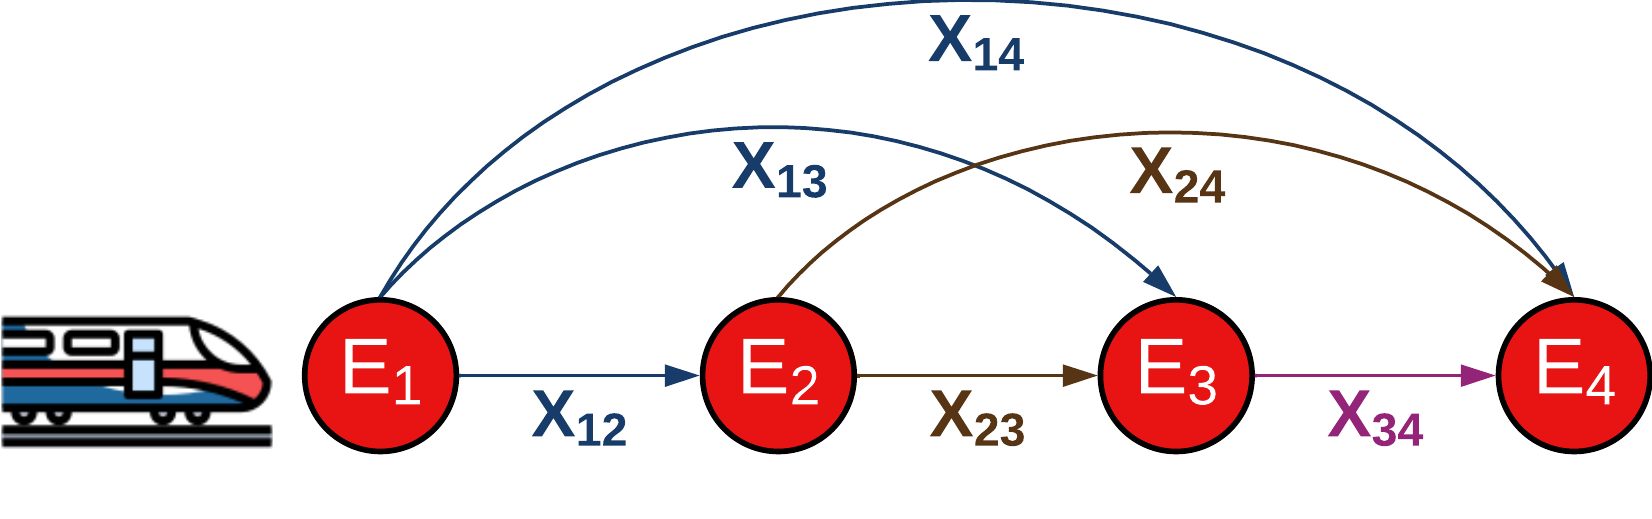
\includegraphics[scale=0.18]{img/repre_ini1.png}
		\caption{Versão gráfica simples}
		% Fonte:~\cite{khaksar2013genetic}}
		\label{fig: fig1}
	\end{center}
\end{figure}


\section{Primeira modelagem matemática}\label{sec:modelo1}

Agora, para a primeira proposta de modelagem, temos o seguinte

\noindent $x_{ij}$: Quantidade de assentos que serão seguradas no trecho com origem em $i$ e destino em $j$, onde $j>i$ (variavel de decisão). \\
\noindent $A_i$: Quantidade de assentos vagos na estação $i$. \\
\noindent $P_{ij}$: Preço da passagem no trajeto com origem em $i$ e destino em $j$. \\
\noindent $Q$: Capacidade física do trem.

Dado o exposto, a função objetivo será maximizar o lucro para cada possível venda em cada trajeto $i,j$, matematicamente seria:

$FO: max \quad x_{12}P_{12} + x_{13}P_{13} + x_{14}P_{14} + x_{23}P_{23} + x_{24}P_{24} + x_{34}P_{34}$

s.a.

Estação 1: $x_{12} + x_{13} + x_{14} \leq A_1 \quad onde \quad A_1 = Q $ \\
\indent Estação 2: $x_{23} + x_{24}  \leq  A_2 \quad onde \quad A_2 = A_1 - (x_{12} + x_{13} + x_{14}) + x_{12} $ \\
\indent Estação 3: $x_{34} \leq A_3 \quad onde \quad A_3 = A_2 - (x_{23} + x_{24}) + x_{13} + x_{23} $

Note que as restrições são aplicadas para cada uma das três primeiras estações, E1, E2 e E3, já que são as estações que têm pelo menos um destino, e a última estação, E4, é excluída, pois não possui nenhum destino.

Cada uma das restrições leva em consideração o fluxo de pessoas que sairão e entrarão no trem. Levando isso em conta, é necessário calcular a disponibilidade do trem para cada estação. Considere uma solução viável para o modelo, conforme mostrado na figura \ref{fig: fig2}, com uma capacidade total de 100 assentos para um trem.

\begin{figure}[!ht]
	\begin{center}
		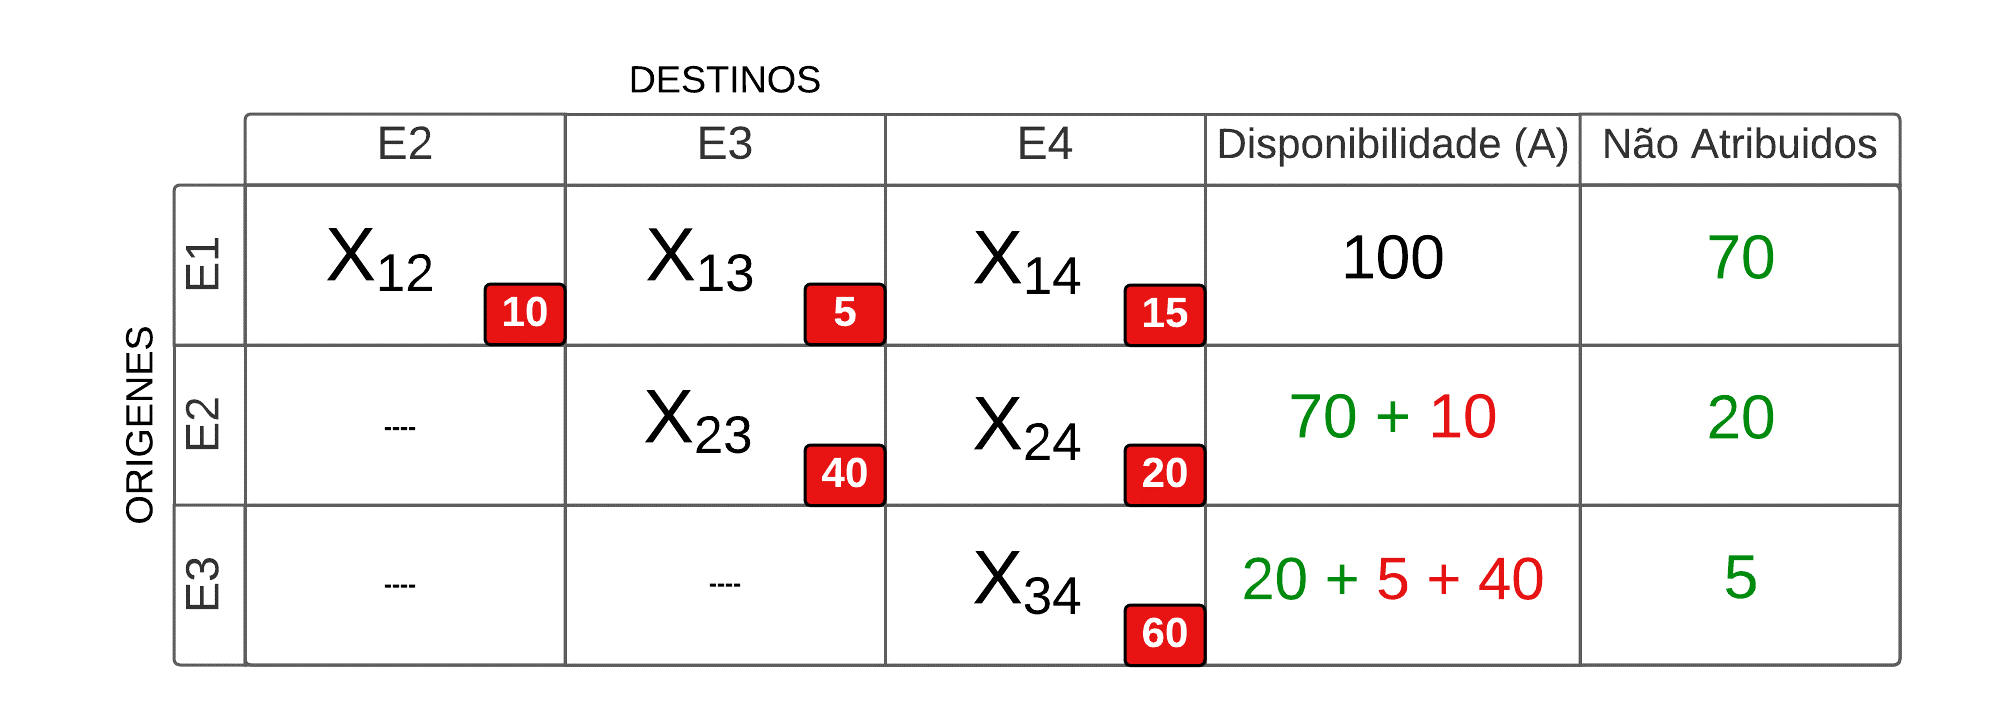
\includegraphics[scale=0.4]{img/fig2.png}
		\caption{Solução factível para o problema simplificado}
		% Fonte:~\cite{khaksar2013genetic}}
		\label{fig: fig2}
	\end{center}
\end{figure}

Note que, para a restrição da estação 1, o trem está com todos os assentos vazios, ou seja, \(A_1=100\), e que a soma das variáveis seria \(x_{12} + x_{13} + x_{14} = 10 + 5 + 15 = 30\). Portanto, teríamos \(30 \leq 100\), ou seja, foram disponibilizados para venda 30 assentos dos 100 que o trem possui. Nesse sentido, no momento da partida do trem da estação 1, haveria 70 assentos vazios ou disponíveis para venda em estações posteriores.

Agora, para a estação 2, teríamos \(A_2 = 100 - 30 + 10 = 70 + 10 = 80\). Já era conhecido que havia 70 assentos disponíveis vindos da estação 1, mas também é preciso levar em conta que os assentos com destino à estação 2 também ficarão disponíveis da estação 2 em diante, para este caso \(x_{12} = 10\). Portanto, para a estação 2, teríamos 80 assentos vazios para disponibilizar, ou seja, \(60 \leq 80\). Analogamente, o mesmo raciocínio seria aplicado para a estação 3, ou seja, teríamos a soma de todos os assentos que chegaram à estação 3, \(x_{13} = 5\) e \(x_{23} = 40\), assim teríamos \(A_3 = 80 - 60 + 5 + 40 = 20 + 5 + 40 = 65\), e no final teríamos \(60 \leq 65\).

Além da lógica anterior, assume-se que há um trem, com vários vagões ou cabines, que viajará de uma estação $E_1$ até uma estação $E_n$ (onde $n$ é a última estação onde o trem chegará). Esse trem terá um itinerário que conterá o nome do trem, a estação de origem, a estação de destino, a data e hora de partida e de chegada. Além disso, haverá uma lista de preços (para o mesmo tipo de assento) a ser disponibilizada para venda. Cada um dos preços da lista será chamado de classe de controle ou control class. Os bilhetes serão disponibilizados para venda antes da partida do trem, e o tempo entre a disponibilização e a referida partida será chamado de horizonte de reserva. Esse horizonte será dividido em vários períodos, que podem ter diferentes temporalidades. Por exemplo, pode haver períodos em dias, semanas, meses, etc., e combinações entre eles. Cada um desses períodos será chamado de check point.

Cada relação possível entre uma estação e outra será denominada origem-destino ou trecho. Será dito que uma origem-destino é adjacente se, e somente se, não houver estações intermediárias entre elas; caso contrário, serão não adjacentes. Por exemplo, na figura \ref{fig: fig1}, os trechos adjacentes seriam: E1-E2, E2-E3, E3-E4, e os trechos não adjacentes seriam: E1-E3, E1-E4 e E2-E4. Além disso, observe que os trechos não adjacentes podem conter outros trechos, tanto adjacentes quanto não adjacentes. Por exemplo, o trecho E1-E4 da figura \ref{fig: fig1} contém os trechos adjacentes E1-E2, E2-E3, e contém os trechos não adjacentes E1-E3 e E2-E4.

Vejamos agora o modelo proposto completo:

\begin{table}[H]
	\centering
	\small
	\begin{tabular}{p{2cm} p{9.5cm} p{3.2cm}}
		\toprule
		\textbf{Definição} & \textbf{Descrição}                                                                                                                                            & \textbf{Domínio}                             \\ \midrule
		\multicolumn{3}{l}{\textbf{Conjuntos}}                                                                                                                                                                                          \\ \midrule
		$O$                & Conjunto de Estações de origem                                                                                                                          &                                              \\
		$D$                & Conjunto de Estações de Destino                                                                                                                          &                                              \\
		$OD$               & Conjunto de Trechos com itinerario                                                                                                                          &                                              \\
		$NAD$              & Conjunto de Trechos que NÃO são Adjacentes e que tem itinerario                                                                                             &                                              \\
		$BRI_{(o,d)}$      & Conjunto de Trechos contidos dentro de cada trecho $(o,d)$ NÃO Adjacente                                                                                    &                                              \\
		$V$                & Conjunto de Cabines do trem                                                                                                                                 &                                              \\
		$T$                & Conjunto de Check-Points (Períodos)                                                                                                                         &                                              \\ 
		$K_v$              & É o conjunto de classes de controle para cada vagão $v$. Por exemplo, suponha que há duas cabines $z$ e $p$, e cada cabine contém três classes de controle $c_1, c_2, c_3$, então a representação seria $K_z:\{c_1,c_2,c_3\}$ e $K_p:\{c_1,c_2,c_3\}$. Além disso, considere que os elementos de cada $K_v$ são ordenados, onde sempre se cumpre que a classe de menor indice é a classe mais costosa, ou seja $c_1>c_2>c_3$.                                                                                                        &                                              \\ \midrule
		\multicolumn{3}{l}{\textbf{Parâmetros}}                                                                                                                                                                                         \\ \midrule
		$n$                & Quantidade de Estações                                                                                                                                                 &                                              \\
		$Q$                & Capacidade física do trem                                                                                                                                          &                                              \\
		$P_{ijvk}$         & Preços  das passagem no Trecho $(i,j)$, Cabine $v$ e Classe de Control $k$                                                                                  & $(i,j) \in OD,v \in V, k \in K_v$            \\
		$d_{ijvkt}$        & Demanda no Trecho $(i,j)$, Cabine $v$ e Classe de Control $k$                                                                                 & $(i,j) \in OD,v \in V, k \in K_v, t \in T$   \\ \midrule
		\multicolumn{3}{l}{\textbf{Variáveis de decisão}}                                                                                                                                                                               \\ \midrule
		$X_{ijvkt}$        & Quantidade de passagem atribuídos no trecho $(i,j)$, cabine $v$ e com classe de control $k$ no período $t$                                                  & $(i,j) \in OD, v \in V, k \in K_v, t \in T$  \\
		$Y_{ijvkt}$        & Quantidade de passagem autorizados no trecho $(i,j)$, cabine $v$ e com classe de control $k$ no período $t$                                                 & $(i,j) \in OD, v \in V, k \in K_v, t \in T$  \\
		$BNA_{ijvkt}$      & É uma variavel binaria que toma o valor de 1 quando $Y_{ijvkt} \neq 0$ e toma  valor de 0 caso contrario, aplica-se apenas a trechos que não são adjacentes & $(i,j) \in NAD, v \in V, k \in K_v, t \in T$ \\\midrule
		\multicolumn{3}{l}{\textbf{Variável auxiliar}}                                                                                                                                                                               \\ \midrule
		$A_{i}$            & Armazena a quantidade de assentos vazios disponíveis para venda em cada estação de origem durante todo o horizonte de reserva. Cabe esclarecer que esta não é uma variável de decisão, pois esta variável apenas armazena um cálculo com base na capacidade física do trem e nas variáveis de decisão de atribuições                                                                                                     & $i \in O$                                    \\
		\bottomrule
	\end{tabular}
	\caption{Notação matemática}
	\label{tab: m1_definicao}
\end{table}

\begin{align}
	& Max \quad Z = \sum_{(i,j)\in OD} \sum_{v\in V} \sum_{k\in K_v} \sum_{t\in T} P_{ijvk} X_{ijvkt}                                                                                                                \label{eq: m1_fo}                          \\
	& \text{s.a.}  \notag                                                                                                                                                                                                                                       \\
	& A_{i} = A_{i-1} - \sum_{(i,j) \in OD/j \geq i} \sum_{v\in V} \sum_{k\in K_v}\sum_{t\in T}X_{i-1,j,v,k,t} + \sum_{(i,j) \in OD/j<i}\sum_{v\in V} \sum_{k\in K_v}\sum_{t\in T}X_{jivkt}, \quad \forall i \in O  \label{eq: m1_disponi}                     \\
	& \sum_{(i,j) \in OD}\sum_{v\in V} \sum_{k\in K_v}\sum_{t\in T} X_{ijvkt} \leq A_{i} , \quad \forall i \in O /i<j, i < n                                                                                        \label{eq: m1_cap_assig}                   \\
	& Y_{ijvkt} \geq Y_{i,j,v,k+1,t},  \quad \forall (i,j) \in OD / i < j, v \in V, k \in K_v / k < \lVert K_v \rVert , t \in T                                                                                                                     \label{eq: m1_jerar_class}                 \\   % P_{ijvk} \geq P_{i,j,v,k+1}
	& X_{ijvkt} \leq d_{ijvkt},  \quad \forall (i,j) \in OD / i < j  ,v \in V, k \in K_v, t\in T                                                                                                                                                  \label{eq: m1_assig_menor_dem}             \\
	& \sum_{(i,j) \in OD}\sum_{v\in V}\sum_{t\in T} Y_{i,j,v,k,t} \leq Q, \quad  k = min\{K_v\}, \forall i \in O                                                                                                  \label{eq: m1_cap_autho_1er_class}         \\
	& Y_{i,j,v,k,t} \geq  X_{i,j,v,k,t},  \quad k = max\{K_v\}, \forall(i,j) \in OD ,v \in V, t \in T                                                                                                                                     \label{eq: m1_autho_mayor_assig_1er_class} \\
	& Y_{i,j,v,k,t} \geq  X_{i,j,v,k,t} + Y_{i,j,v,k + 1,t} , \forall(i,j) \in OD, v \in V, k \in K_v / k < \lVert K_v \rVert , t \in T                                                                                                            \label{eq: m1_autho_mayor_assig_mas_autho} \\
	& BNA_{o,d,v,k,t} \leq Y_{o,d,v,k,t} \leq BNA_{o,d,v,k,t} Q, \quad  \forall (o,d)\in NAD, v \in V, k \in K_v, t \in T                                                                                                                \label{eq: m1_activ_bin_autho}            \\
	& BNA_{o,d,v,k,t} \leq Y_{i,j,v,k,t} \leq BNA_{o,d,v,k,t} Q, \quad  \forall (o,d)\in NAD, (i,j) \in BRI_{(o,d)}, v \in V, k \in K_v, t \in T                                                                                            \label{eq: m1_autho_igualar_trecho_maior}  \\
	& X_{0,j,v,k,t} = 0,     \quad \forall j \in D, k \in K_v, t \in T                                                                                                                                                                     \label{eq: m1_ini_assig}                   \\
	& A_{0} = Q                                                                                                                                                                                                      \label{eq: m1_ini_disponi}                 \\
	& X_{ijvkt} \in \mathbb{Z}^+                                                                                                                                                                                     \label{eq: m1_dom_assig}                   \\
	& Y_{ijvkt} \in \mathbb{Z}^+                                                                                                                                                                                     \label{eq: m1_dom_autho}                   \\
	& A_{j} \in \mathbb{Z}^+                                                                                                                                                                                         \label{eq: m1_dom_disponi}                 \\
	& BNA_{ijvkt} \in \{0,1\}                                                                                                                                                                                        \label{eq: m1_dom_bin_nadja}
\end{align}
% \begin{align}      
% 	& Y_{i,j,v,k,t} \geq  X_{i,j,v,k,t},  \quad k = max\{K_v\}, \forall(i,j),v,t                                                                                                                                     \label{eq: m1_autho_mayor_assig_1er_class} \\
% 	& Y_{i,j,v,k,t} \geq  X_{i,j,v,k,t} + Y_{i,j,v,k + 1,t} , \forall(i,j),v, k, t / k < \lVert K_v\rVert                                                                                                            \label{eq: m1_autho_mayor_assig_mas_autho} \\
% 	& BNA_{o,d,v,k,t} \leq Y_{o,d,v,k,t} \leq BNA_{o,d,v,k,t} Q, \quad  \forall (o,d)\in NAD, v, k, t                                                                                                                \label{eq: m1_activ_bin_autho}             \\
% 	& BNA_{o,d,v,k,t} \leq Y_{i,j,v,k,t} \leq BNA_{o,d,v,k,t} Q, \quad  \forall (o,d)\in NAD, (i,j) \in BRI_{(o,d)}, v,k,t                                                                                           \label{eq: m1_autho_igualar_trecho_maior}  \\
% 	& X_{0,j,v,k,t} = 0,     \quad \forall j,k,t                                                                                                                                                                     \label{eq: m1_ini_assig}                   \\
% 	& A_{0} = Q                                                                                                                                                                                                      \label{eq: m1_ini_disponi}                 \\
% 	& X_{ijvkt} \in \mathbb{Z}^+                                                                                                                                                                                     \label{eq: m1_dom_assig}                   \\
% 	& Y_{ijvkt} \in \mathbb{Z}^+                                                                                                                                                                                     \label{eq: m1_dom_autho}                   \\
% 	& A_{j} \in \mathbb{Z}^+                                                                                                                                                                                         \label{eq: m1_dom_disponi}                 \\
% 	& BNA_{ijvkt} \in \{0,1\}                                                                                                                                                                                        \label{eq: m1_dom_bin_nadja}
% \end{align}


Na equação \ref{eq: m1_fo}, a qual representa a função objetivo, temos a soma do produto entre a quantidade de assentos atribuídos a cada trajeto de origem e destino para a classe comercial em cada período e cada vagão, multiplicada pelo preço correspondente para cada trajeto e classe. Observe que queremos maximizar os ingressos em função dos assentos que estão atribuídos, que é o mais próximo que se tem da realidade em função da demanda conhecida.

A restrição \ref{eq: m1_disponi} é utilizada para calcular a disponibilidade de assentos de cada estação de origem, em cada período de tempo para cada classe em cada vagão e é a generalização do exemplo simplificado para calcular a variável auxiliar $A_i$.

A restrição \ref{eq: m1_cap_assig} garante que todas as autorizações habilitadas a partir de cada estação de origem para cada período e cada classe de cada vagão não excedam a disponibilidade da sua estação de origem correspondente (a disponibilidades é calculada na restrição \ref{eq: m1_disponi}).

A restrição \ref{eq: m1_jerar_class} é uma restrição de hierarquia e garante que as quantidades de autorizações para as classes de maior preço sejam sempre maiores do que as quantidades de autorizações de menor preço em cada vagão, em cada trecho, e em  cada período do horizonte de reserva.

A restrição \ref{eq: m1_assig_menor_dem} garante que a quantidade de atribuições não ultrapasse a demanda para cada trecho de cada classe em cada vagoen e em cada período no horizonte de reserva.

A restrição \ref{eq: m1_cap_autho_1er_class} garanta que a soma de autorizações da classe mais costosa de cada vagão, de cada estação de origem, de tudos os periodos, não ultrapase a capacidade do trem, note que apenas estamos considerando a classe mais cara devido à natureza cumulativa das variáveis de autorização é por isso que o valor de k é o mínimo das classes de cada vagão, pois a ordem do nome das classes é crescente mas o seu valor é decrescente. Para melhor compreensão, suponhamos uma solução para um problema de dois vagões $V_1$ e $V_2$, 3 classes para $V_1$ e 3 classes para $V_2$, 5 estações,  10 trechos, um período e uma capacidade física do trem de 700 cadeiras, conforme mostra a figura \ref{fig: autorization}.

\begin{figure}[!ht]
	\begin{center}
		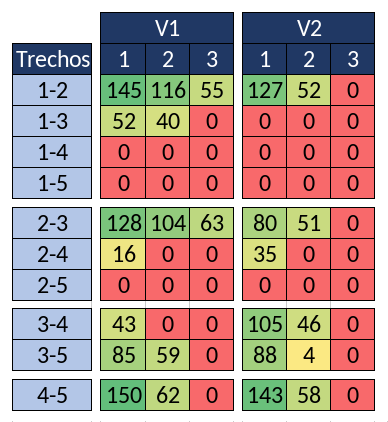
\includegraphics[scale=0.40]{img/exemplo1.png}
		\caption{Solução factível para a variavel de desição Autorização}
		% Fonte:~\cite{khaksar2013genetic}}
		\label{fig: autorization}
	\end{center}
\end{figure}

Observe que os nomes das classes são números ordenados de forma crescente [1, 2, 3] também o valor da classe 1 é mais caro que o valor da classe 2 e este é maior que o valor da classe 3. Além disso, a soma que não ultrapassará a capacidade do trem é a soma das classes 1 de cada vagão de cada estação de origem. Por exemplo, para a estação 3 seria $43 + 85$ para $V_1$ trecho 3-4 e 3-5, mais, $105 + 88$ para $V_2$ nos mesmos trechos, ou seja $43 + 85 + 105 + 88 = 321 \leq 700$  


Até ao momento foi referido que a variável $Y$ tem um carácter cumulativo e são as restrições \ref{eq: m1_autho_mayor_assig_1er_class} e \ref{eq: m1_autho_mayor_assig_mas_autho} que controlam este comportamento. A restrição \ref{eq: m1_autho_mayor_assig_1er_class} é um caso particular da restrição \ref{eq: m1_autho_mayor_assig_mas_autho}, aplicada apenas à última classe, ou classe mais barata atribuída para cada vagão ($k=max\{K_v\}$), e garante que a soma de todos os períodos, de cada estação de origem da classe mais barata da variável "autorização" é maior ou igual à variável de decisão "segurada" nas mesmas condições. Por outro lado, a restrição \ref{eq: m1_autho_mayor_assig_mas_autho} garante que cada classe autorizada seja sempre maior ou igual à classe autorizada imediatamente menor, mais a quantidade segurada da mesma classe, isto para cada período, cada trecho e cada classe diferente da classe mais barata. Para melhor compreensão, assuma as mesmas suposições que foram feitas na restrição \ref{eq: m1_cap_autho_1er_class} %com a diferença que agora as tabelas representam uma solução factivel para a soma de n períodos e não um único período.


\begin{figure}[h!]
	\centering
	\begin{subfigure}[b]{0.35\linewidth}
		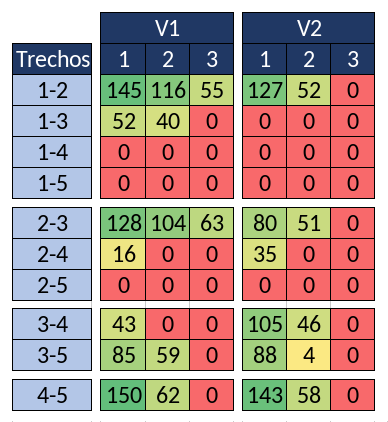
\includegraphics[width=\linewidth]{img/exemplo1.png}
		\caption{Autorização [Variavel $Y$]}
		\label{fig:auto_assig_a}
	\end{subfigure}\hspace{5mm}
	\begin{subfigure}[b]{0.35\linewidth}
		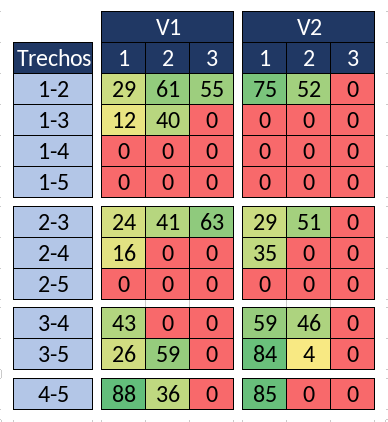
\includegraphics[width=\linewidth]{img/exemplo2.png}
		\caption{Atribução [Variavel $X$]}
		\label{fig:auto_assig_b}
	\end{subfigure}
	\caption{Solução factível para as variaveis de desição Autorização e Atribução}
	\label{fig:auto_assig}
\end{figure}

Observe a linha correspondente ao trecho 1-2 do vagão $V_2$ na tabela \ref{fig:auto_assig_b}, veja que a classe segurada mais barata foi a classe 2 com valor de 52, por este motivo na tabela \ref{fig:auto_assig_a} na mesma posição o valor deverá ser igual ou maior que 52, que neste caso é o mesmo valor; Agora observe para o mesmo trecho para o vagão $V_1$ classe 3 em ambas as tabelas acontece a mesma coisa, esse comportamento é garantido pela restrição \ref{eq: m1_autho_mayor_assig_1er_class}. Agora não vamos olhar para a classe mais barata, vamos olhar para qualquer outra, por exemplo, para o mesmo trecho veja a classe 1 do vagão $V_1$ da tabela \ref{fig:auto_assig_b} com valor 29, se quiséssemos saber o valor correspondente na tabela \ref{fig:auto_assig_a} deveríamos adicionar a classe imediata menor (à direita) da classe 1 na tabela \ref{fig:auto_assig_a}, neste caso seria a classe 2 com valor 116, e some o valor da classe 1 da tabela \ref{fig:auto_assig_b}, que já sabemos que é 29, assim, o valor buscado será maior ou igual a $116+29 = 145$, como visto em tabela \ref{fig:auto_assig_a}, lembre-se que nessa posição o valor mínimo será o calculado, mas poderá assumir um valor superior. Esta última situação é controlada pela restrição \ref{eq: m1_autho_mayor_assig_mas_autho}.

Suponha que você tem um trecho não adjacente E1-E3, e que esse trecho contém outros trechos E1-E2 e E2-E3. Para esta situação, a classe mais barata ativada no trecho E1-E3 deverá ser a classe mais barata ativada nos trechos E1-E2 e E2-E3. Isso é feito com o objetivo de que as combinações dos preços dos bilhetes por trechos não sejam mais econômicos do que o preço de um bilhete direto. Para alcançar isso, é criada uma variável binária para cada trecho não adjacente ($BNA$), que será ativada, ou tomará o valor de 1, quando as atribuições $"Y"$ (ou assentos a serem disponibilizados para venda) de uma classe desse trecho, de um vagão e de um período, forem diferentes de zero e tomará o valor de zero caso contrário. Esse comportamento será controlado pela restrição \ref{eq: m1_activ_bin_autho}.

Uma vez calculados os valores para $BNA$ dos trechos não adjacentes, a restrição \ref{eq: m1_autho_igualar_trecho_maior} fará com que as classes de controle de todos os trechos contidos em cada trecho não adjacente sejam $0$ ou, no mínimo $1$. Assim, quando a classe de controle do trecho não adjacente assumir um valor de $BNA = 0$, essa classe será $0$ para os trechos contidos. Por outro lado, se a classe de controle do trecho não adjacente assumir o valor de $BNA = 1$, então essa classe tomará, no mínimo, o valor de $1$ para todos os trechos contidos.

Para um melhor entendimento, suponha um trem com 1 vagão que passa por 3 estações, $E_1$, $E_2$ e $E_3$, e tem um horizonte de reserva de um único período. Sob esta situação, o trecho não adjacente seria $"E_1-E_3"$ e os trechos contidos seriam $"E_1-E_2"$ e $"E_2-E_3"$. Agora imagine que cada trecho tem 6 classes diferentes ($c_1, c_2, c_3, c_4, c_5, c_6$), onde o preço  de  $c_1 \geq c_2 \geq c_3 \geq c_4 \geq c_5 \geq c_6$, e que as autorizações (variavel $Y$) tomam os valores mostrados na tabela \ref{fig: exemplo_sip}:

\begin{figure}[!ht]
	\begin{center}
		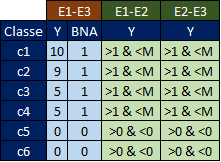
\includegraphics[scale=0.8]{img/tab_trechos_maiores.png}
		\caption{Exemplo simplificado do funcionamento da restrição \ref{eq: m1_autho_igualar_trecho_maior}}
		% Fonte:~\cite{khaksar2013genetic}}
		\label{fig: exemplo_sip}
	\end{center}
\end{figure}

Para o trecho $"E_1-E_3"$, note que quando $Y \neq 0$, $BNA = 1$ e quando $Y = 0$, $BNA = 0$ (controlado pela restrição \ref{eq: m1_activ_bin_autho}). Agora observe que, quando $ BNA = 1$ para uma certa classe, os trechos $E_1-E_2$ e $E_2-E_3$ assumem valores entre 1 e um número suficientemente grande ($1 \le Y \leq M$), o que indica que os assentos a serem disponibilizados para essa classe nesses trechos não podem ser zero. Por outro lado, quando $BNA = 0$, os trechos menores devem zerar a classe correspondente com ($0 \leq Y \leq 0$), ou seja, não se deve disponibilizar assentos com essa classe (controlado pela restrição \ref{eq: m1_autho_igualar_trecho_maior}). Deve-se esclarecer que as classe de controle dos trechos contidos, apenas imitam o comportamento da classe não adjacente correspondente, e não os valores que esta assume.

As restrições de \ref{eq: m1_ini_assig} e \ref{eq: m1_ini_disponi} são usadas para inicializar a restrição \ref{eq: m1_disponi} quando \(i = 1\). E as restrições de \ref{eq: m1_dom_assig} a \ref{eq: m1_dom_bin_nadja} representam o domínio das variáveis.

\section{Segunda modelagem matemática}\label{sec:modelo2}

Vamos considerar novamente uma versão simplificada do problema. Na verdade, para esta modelagem, serão levadas em conta as mesmas variáveis do primeiro modelo, exceto a variável de disponibilidade \(A\), conforme mostrado a seguir:

\noindent $x_{ij}$: Quantidade de assentos que será disponibilizada para venda no trecho com origem em $i$ e destino em $j$, onde $j>i$ \\
\noindent $P_{ij}$: Preço da passagem no trajeto com origem em $i$ e destino em $j$ \\
\noindent $Q$: Capacidade do trem

\noindent Assim, a função objetivo e as restrições são como segue:

$FO: max \quad x_{12}P_{12} + x_{13}P_{13} + x_{14}P_{14} + x_{23}P_{23} + x_{24}P_{24} + x_{34}P_{34}$

s.a.

\noindent{\it Restrições para estações de origem}

Estação 1: $x_{12} + x_{13} + x_{14} \leq Q $ \\
\indent Estação 2: $x_{23} + x_{24}  \leq  Q $ \\
\indent Estação 3: $x_{34} \leq Q $

\noindent{\it Restrições para estações de destino}

Estação 2: $x_{12} \leq Q $ \\
\indent Estação 3: $x_{13} + x_{23}  \leq  Q $ \\
\indent Estação 4: $x_{14} + x_{24} + x_{34} \leq Q $

Observe que esta formulação é baseada nos modelos de transporte, onde as estações de origem seriam os depósitos e estão restritas por sua capacidade (capacidade do trem), e as estações de destino seriam os destinos e estão restritas, neste caso, pela mesma capacidade do trem e não pela demanda de cada destino.

Esta formulação garante que sempre será disponibilizada, no máximo, a capacidade do trem tanto para cada saída quanto para cada chegada do trem. Imagine uma solução viável como a mostrada na figura \ref{fig: fig2}.

\begin{figure}[h]
	\begin{center}
		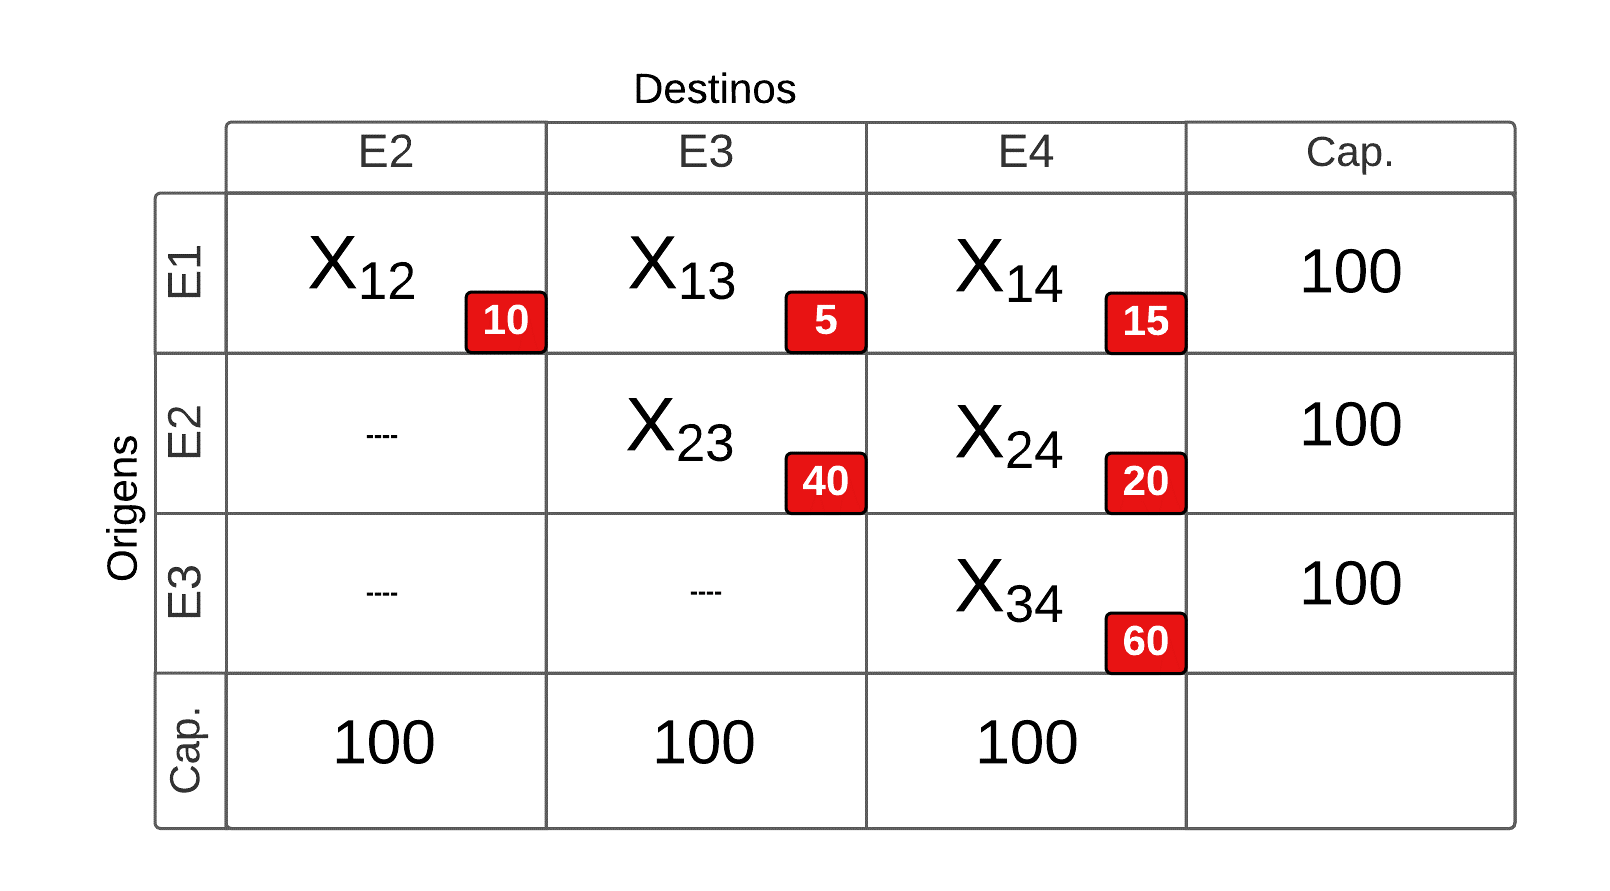
\includegraphics[scale=0.4]{img/fig3.png}
		\caption{Solução factível para o problema simplificado}
		% Fonte:~\cite{khaksar2013genetic}}
		\label{fig: fig3}
	\end{center}
\end{figure}

Observe que os valores das variáveis são os mesmos que foram mostrados na figura \ref{fig: fig3}. E ainda todas as restrições, tanto por linha quanto por coluna (por origens e por destinos), continuam sendo atendidas.

\begin{table}[h]
	\centering
	\small
	\begin{tabular}{p{2cm} p{9.5cm} p{3.2cm}}
		\toprule
		\textbf{Definição} & \textbf{Notação}                                                                                                                                            & \textbf{Domínio}                             \\ \midrule
		\multicolumn{3}{l}{\textbf{Conjuntos}}                                                                                                                                                                                          \\ \midrule
		$OD$               & Conjunto de Trechos com itinerario                                                                                                                          &                                              \\
		$NAD$              & Conjunto de Trechos que NÃO são Adjacentes e que tem itinerario                                                                                             &                                              \\
		$BRI_{(o,d)}$      & Conjunto de Trechos contidos dentro de cada trecho $(o,d)$ NÃO Adjacente                                                                                    &                                              \\
		$V$                & Conjunto de Cabines do trem                                                                                                                                 &                                              \\
		$K_v$              & Conjunto de Classes de Control de cada cabine em $V$                                                                                                        &                                              \\
		$T$                & Conjunto de Check-Points (Períodos)                                                                                                                         &                                              \\ \midrule
		\multicolumn{3}{l}{\textbf{Parâmetros}}                                                                                                                                                                                         \\ \midrule
		$Q$                & Capacidade do trem                                                                                                                                          &                                              \\
		$P_{ijvk}$         & Preços  das passagem no Trecho $(i,j)$, Cabine $v$ e Classe de Control $k$                                                                                  & $(i,j) \in OD,v \in V, k \in K_v$            \\
		$D_{ijvkt}$        & Demanda  das passagem no Trecho $(i,j)$, Cabine $v$ e Classe de Control $k$                                                                                 & $(i,j) \in OD,v \in V, k \in K_v, t \in T$   \\ \midrule
		\multicolumn{3}{l}{\textbf{Variáveis de decisão}}                                                                                                                                                                               \\ \midrule
		$X_{ijvkt}$        & Quantidade de passagem atribuídos no trecho $(i,j)$, cabine $v$ e com classe de control $k$ no período $t$                                                  & $(i,j) \in OD, v \in V, k \in K_v, t \in T$  \\
		$Y_{ijvkt}$        & Quantidade de passagem autorizados no trecho $(i,j)$, cabine $v$ e com classe de control $k$ no período $t$                                                 & $(i,j) \in OD, v \in V, k \in K_v, t \in T$  \\
		$BNA_{ijvkt}$      & É uma variavel binaria que toma o valor de 1 quando $Y_{ijvkt} \neq 0$ e toma  valor de 0 caso contrario, aplica-se apenas a trechos que não são adjacentes & $(i,j) \in NAD, v \in V, k \in K_v, t \in T$ \\
		\bottomrule
	\end{tabular}
	\caption{Notação matemática}
	\label{tab: m2_definicao}
\end{table}
\begin{align}
	 & Max \quad Z = \sum_{(i,j)\in OD} \sum_{v\in V} \sum_{k\in K_v} \sum_{t\in T} P_{ijvk} X_{ijvkt}                                 \label{eq: m2_fo}                          \\
	 & \text{s.a.}  \notag                                                                                                                                                        \\
	 & \sum_{(i,j)\in OD}\sum_{v\in V}\sum_{k\in K_v}\sum_{t\in T}X_{ijvkt} \leq Q , \quad \forall j / j>1, i<j                        \label{eq: m2_cap_assig_destino}           \\
	 & \sum_{(i,j)\in OD}\sum_{v\in V}\sum_{k\in K_v}\sum_{t\in T}X_{ijvkt} \leq Q , \quad \forall i / i<n, j>i                        \label{eq: m2_cap_assig_origem}            \\
	 & Y_{ijvkt} \geq Y_{i,j,v,k+1,t},  \quad \forall (i,j),v,k,t / i < j, k < \lVert K_v \rVert,  P_{ijvk} \geq P_{i,j,v,k+1}         \label{eq: m2_jerar_class}                 \\
	 & X_{ijvkt} \leq D_{ijvkt},  \quad \forall (i,j),v,k,t/ i < j                                                                     \label{eq: m2_assig_menor_dem}             \\
	 & \sum_{(i,j) \in OD}\sum_{v\in V}\sum_{t\in T} Y_{i,j,v,k,t} \leq Q, \quad  k = min\{K_v\}, \forall i \in OD                     \label{eq: m2_cap_autho_1er_class}         \\
	 & Y_{i,j,v,k,t} \geq  X_{i,j,v,k,t},  \quad k = max\{K_v\}, \forall(i,j),v,t                                                      \label{eq: m2_autho_mayor_assig_1er_class} \\
	 & Y_{i,j,v,k,t} \geq  X_{i,j,v,k,t} + Y_{i,j,v,k + 1,t} , \forall(i,j),v, k, t / k < \lVert K_v\rVert                             \label{eq: m2_autho_mayor_assig_mas_autho} %\\
	%  & BNA_{o,d,v,k,t} \leq Y_{o,d,v,k,t} \leq BNA_{o,d,v,k,t} Q, \quad  \forall (o,d)\in NAD, v, k, t                                 \label{eq: m2_activ_bin_autho}             \\
	%  & BNA_{o,d,v,k,t} \leq Y_{i,j,v,k,t} \leq BNA_{o,d,v,k,t} Q, \quad  \forall (o,d)\in NAD, (i,j) \in BRI_{(o,d)}, v,k,t            \label{eq: m2_autho_igualar_trecho_maior}  \\
	%  & X_{ijvkt} \in \mathbb{Z}^+                                                                                                      \label{eq: m2_dom_assig}                  %\\
\end{align}
\begin{align}
	& BNA_{o,d,v,k,t} \leq Y_{o,d,v,k,t} \leq BNA_{o,d,v,k,t} Q, \quad  \forall (o,d)\in NAD, v, k, t                                 \label{eq: m2_activ_bin_autho}             \\
	& BNA_{o,d,v,k,t} \leq Y_{i,j,v,k,t} \leq BNA_{o,d,v,k,t} Q, \quad  \forall (o,d)\in NAD, (i,j) \in BRI_{(o,d)}, v,k,t            \label{eq: m2_autho_igualar_trecho_maior}  \\
	& X_{ijvkt} \in \mathbb{Z}^+                                                                                                      \label{eq: m2_dom_assig}                   \\
	& Y_{ijvkt} \in \mathbb{Z}^+                                                                                                      \label{eq: m2_dom_autho}                   \\
	& BNA_{ijvkt} \in \{0,1\}                                                                                                         \label{eq: m2_dom_bin_nadja}
\end{align}

Como já foi mencionado, nesta formulação modificamos as restrições que controlam as variáveis asseguradas X, ou seja, mudamos as restrições 1 e 2 do primeiro modelo e eliminamos a variável de decisão Ai.

% \end{adjustwidth}
%Note que, na definição, não temos mais a variável de decisão de disponibilidade \(A_i\). Neste caso, a equação \ref{eq: m2_fo} representa a função objetivo que esta tentando maximizar a soma do produto entre as quantidades seguradas e os preços das mesmas, ou seja, estamos maximizando a receita em função das quantidades dos assentos que estão assegurados.

%A restrição \ref{eq: m2_cap_assig_destino} garante que a quantidade total de assentos autorizados para cada destino seja a quantidade máxima de assentos do trem para todas as classes e todos os períodos.
%A restrição \ref{eq: m2_cap_assig_origem} garante que a quantidade de assentos autorizados para cada origem seja no máximo a capacidade do trem para todas as classes e todos os períodos.
%As restrições de \ref{eq: m2_cap_autho_1er_class} a \ref{eq: m2_dom_autho} representam o mesmo que o primeiro modelo já exposto.\\

Para este caso, as restrições \ref{eq: m2_cap_assig_destino} e \ref{eq: m2_cap_assig_origem} representam a generalização do problema simplificado, onde a primeira garante que a quantidade de assentos autorizados para venda não viole a capacidade do trem ao chegar a cada estação de destino; e a segunda garante que a quantidade de assentos autorizados respeite a capacidade do trem no momento de sair de cada estação de origem. O restante das restrições foi explicado na formulação 1.
% \input{Contribuicoes}
% %\input{Metodos-de-resolucao-propostos}
% \input{Resultados-computacionais}
% \input{Conclusoes}



% %=============================== Referências Bibliográficas===========================
% \addcontentsline{toc}{chapter}{Bibliografia}\label{referencias}
% \bibliographystyle{agsm}
% \bibliography{referencias}




% %=============================== Anexos ==========================
% \appendix
% \renewcommand{\appendixname}{Appendix} %trocar Apendice por Anexo
% \include{G-Appendix}

\end{document}